\documentclass[]{elementary-physics}

\usepackage{circuitikz}

\title{1. Masses Combined in Series and in Parallel}
\date{2015-05-10 v4.9}

\begin{document}

\maketitle

\tableofcontents

\section{Abstract}

When masses are combined in the natural way as in $m_c = m_1 + m_2$ they have the same velocity and are thus combined in series.
During an elastic collision with a spring the masses experience the same amount of force and are thus combined in parallel as in $m^{-1}_c = m^{-1}_1 + m^{-1}_2$ from the perspective of the spring. \directlua{hello = "hi there";tex.print(hello)}

\section{Collision}

We believe the easiest way to describe masses combined in parallel is to compare them to capacitors in series.
During this comparison\cite{wpana} we compare mass to capacitance, spring to inductance, velocity to voltage and momentum to charge.\directlua{tex.print(hello)}

In this example the two masses have the following properties:

\begin{figure}[ht] \centering
	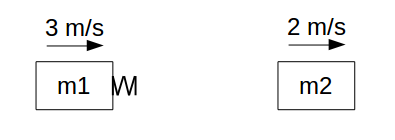
\includegraphics[scale=.5]{mms1} \caption{Masses initial state}
\end{figure}

\begin{subequations}
\begin{align}
m_1 &= 2 \, kg \\
v_1 &= 3 \, m/s \\
p_1 &= 6 \, kg \, m/s \\
m_2 &= 3 \, kg \\
v_2 &= 2 \, m/s \\
p_2 &= 6 \, kg \, m/s
\end{align}
\end{subequations}

The corresponding values for the capacitors would then be:

\begin{figure}[ht] \centering
		\begin{circuitikz}
			\draw
				(0,0) to[C=2\si{\farad},v>=3\si{\volt}] 
				(0,2) to[switch]
				(2,2) to[L]
				(4,2) to[C=3\si{\farad},v<=2\si{\volt}]
				(4,0) -- (0,0);
		\end{circuitikz}
	\caption{Tvo Capacitors, initial state}
\end{figure}

%\begin{figure}[ht] \centering
%	\subfloat[Two capacitors]
%		{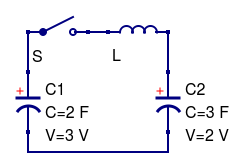
\includegraphics[scale=.5]{ccl1} \label{sf1}}
%	\qquad
%	\subfloat[One capacitor]
%		{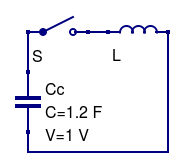
\includegraphics[scale=.5]{ccl1c} \label{sf2}}
%	\caption{Capacitors' initial state}
%\end{figure}

\begin{subequations}
\begin{align}
C_1 &= 2 \, \si{\farad} \\
V_1 &= 3 \, \si{\volt} \\
Q_1 &= 6 \, \si{\coulomb} \\
C_2 &= 3 \, \si{\farad} \\
V_2 &= 2 \, \si{\volt} \\
Q_2 &= 6 \, \si{\coulomb}
\end{align}
\end{subequations}

From the inductor`s point of view, when we close the switch we could replace the two capacitors with one capacitor, just as from the spring`s point of view we could replace the two masses with one:

\begin{figure}[ht] \centering
		\begin{circuitikz}
			\draw
				(0,0) to[C=1.2\si{\farad},v>=1\si{\volt}] 
				(0,2) to[switch]
				(2,2) to[L]
				(4,2) --
				(4,0) -- (0,0);
		\end{circuitikz}
	\caption{One Capacitor, initial state}
\end{figure}

\begin{subequations}
\begin{align}
C_c &= 1/(1/2 + 1/3) = 1.2 \, \si{\farad} \\
V_c &= 3 - 2 = 1 \, \si{\volt} \\
Q_c &= 1.2 * 1 = 1.2 \, \si{\coulomb}
\end{align}
\end{subequations}

If the collision was inelastic it would be as if the inductor was a resistor and the result would be:

%\begin{figure}[ht] \centering
%	\subfloat[Two capacitors]
%		{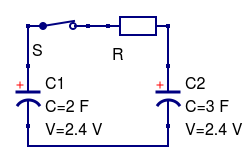
\includegraphics[scale=.5]{ccl2} \label{sf2}}
%	\qquad
%	\subfloat[One capacitor]
%		{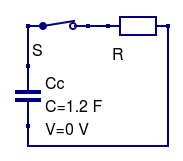
\includegraphics[scale=.5]{ccl2c} \label{sf1}}
%	\caption{Capacitors after 'inelastic collision'}
%\end{figure}

\begin{figure}[ht] \centering
		\begin{circuitikz}
			\draw
				(0,0) to[C=1.2\si{\farad},v>=0\si{\volt}] 
				(0,2) to[opening switch]
				(2,2) to[R]
				(4,2) --
				(4,0) -- (0,0);
		\end{circuitikz}
	\caption{One Capacitor, after 'inelastic collision'}
\end{figure}

\begin{subequations}
\begin{align}
C_c &= 1.2 \, \si{\farad} \\
Q_c &= 1.2 - 1.2 = 0 \, \si{\coulomb} \\
V_c &= 0 \, \si{\volt}
\end{align}
\end{subequations}

Or in the case of two capacitors:

\begin{figure}[ht] \centering
		\begin{circuitikz}
			\draw
				(0,0) to[C=2\si{\farad},v>=2.4\si{\volt}] 
				(0,2) to[opening switch]
				(2,2) to[L]
				(4,2) to[C=3\si{\farad},v<=2.4\si{\volt}]
				(4,0) -- (0,0);
		\end{circuitikz}
	\caption{Tvo Capacitors, after 'inelastic collision'}
\end{figure}

\begin{subequations}
\begin{align}
C_1 &= 2 \, \si{\farad} \\
Q_1 &= 6 - 1.2 = 4.8 \, \si{\coulomb} \\
V_1 &= 4.8 / 2 = 2.4 \, \si{\volt} \\
C_2 &= 3 \, \si{\farad} \\
Q_2 &= 6 + 1.2 = 7.2 \, \si{\coulomb} \\
V_2 &= 7.2 / 3 = 2.4 \, \si{\volt}
\end{align}
\end{subequations}

\begin{figure}[ht] \centering
	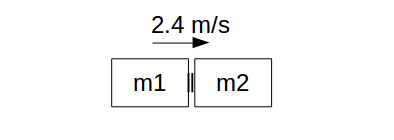
\includegraphics[scale=.5]{mms2} \caption{Masses after inelastic collision}
\end{figure}

What happens is that $1.2 \, \si{\coulomb}$ flows from $C_1$ to $C_2$, or if it
was two masses, momentum is transferred from $m_1$ to $m_2$.\\
\\
But in this case we have an inductor and not a resistor so the energy from the flowing charge is stored in the magnetic field of the inductor.
If it was two masses and a spring, we would have an elastic collision and the energy would be in the tension of the spring.
So what happens now is that another $1.2 \, \si{\coulomb}$ continues to flow
through the inductor as the magnetic field collapses:

%\begin{figure}[ht] \centering
%	\subfloat[Two capacitors]
%		{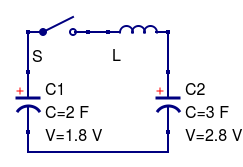
\includegraphics[scale=.5]{ccl3} \label{sf2}}
%	\qquad
%	\subfloat[One capacitor]
%		{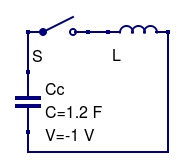
\includegraphics[scale=.5]{ccl3c} \label{sf1}}
%	\caption{Capacitors after 'elastic collision'}
%\end{figure}

\begin{figure}[ht] \centering
		\begin{circuitikz}
			\draw
				(0,0) to[C=1.2\si{\farad},v<=1\si{\volt}] 
				(0,2) to[opening switch]
				(2,2) to[R]
				(4,2) --
				(4,0) -- (0,0);
		\end{circuitikz}
	\caption{One Capacitor, after 'elastic collision'}
\end{figure}

\begin{subequations}
\begin{align}
C_c &= 1.2 \, \si{\farad} \\
Q_c &= 1.2 - 2*1.2 = -1.2 \, \si{\coulomb} \\
V_c &= -1.2 / 1.2 = -1 \, \si{\volt}
\end{align}
\end{subequations}

Or in the case of two capacitors:

\begin{figure}[ht] \centering
		\begin{circuitikz}
			\draw
				(0,0) to[C=2\si{\farad},v>=1.8\si{\volt}] 
				(0,2) to[opening switch]
				(2,2) to[L]
				(4,2) to[C=3\si{\farad},v<=2.8\si{\volt}]
				(4,0) -- (0,0);
		\end{circuitikz}
	\caption{Tvo Capacitors, after 'elastic collision'}
\end{figure}

\begin{subequations}
\begin{align}
C_1 &= 2 \, \si{\farad} \\
Q_1 &= 6 - 2*1.2 = 3.6 \, \si{\coulomb} \\
V_1 &= 3.6 / 2 = 1.8 \, \si{\volt} \\
C_2 &= 3 \, \si{\farad} \\
Q_2 &= 6 + 2*1.2 = 8.4 \, \si{\coulomb} \\
V_2 &= 8.4 / 3 = 2.8 \, \si{\volt} 
\end{align}
\end{subequations}

\begin{figure}[ht] \centering
	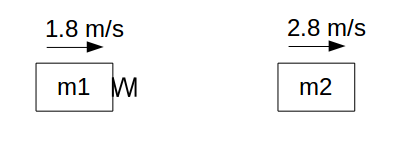
\includegraphics[scale=.5]{mms3} \caption{Masses after elastic collision}
\end{figure}

The corresponding calculations for the masses:

\begin{subequations}
\begin{align}
m_1 &= 2 \, kg \\
p_1 &= 6 - 2*1.2 = 3.6 \, kg \, m/s \\
v_1 &= 3.6 / 2 = 1.8 \, m/s \\
m_2 &= 3 \, kg \\
p_2 &= 6 + 2*1.2 = 8.4 \, kg \, m/s \\
v_2 &= 8.4 / 3 = 2.8 \, m/s 
\end{align}
\end{subequations}

If we hadn't opened the switch we would have an oscillation in the circuit which could be compared to a spring attached to both masses making them oscillate.

\section{Formulas}

\subsection{Inelastic Collision}

The standard way to calculate the new velocity in a completely inelastic collision is this equation where preservation of momentum is used:

\begin{subequations}
\begin{align}
m_1 v_1 + m_2 v_2 &= (m_1 + m_2)v_{new} \\
v_{new} &= \frac{m_1 v_1 + m_2 v_2}{m_1 + m_2}
\end{align}
\end{subequations}

Using our way, first calculate the combination of the masses from the spring`s point of view using the initial velocities:

\begin{subequations}
\begin{align}
m_c &= 1/(1/m_1 + 1/m_2) \\
v_c &= v_1 - v_2 \\
p_c &= m_c v_c
\end{align}
\end{subequations}

Then transfer the combined momentum from either mass $m_1$ or $m_2$ to get its new momentum:

\begin{equation}
{p_1}_{new} = m_1 v_1 - p_c
\end{equation}

Or:

\begin{equation}
{p_2}_{new} = m_2 v_2 + p_c
\end{equation}

And then calculate the new velocity from an observer`s point of view using the new momentum and we get the same result:

\begin{subequations}
\begin{align}
{v}_{new} &= \frac{{p_1}_{new}}{m_1} = \frac{m_1 v_1 + m_2 v_2}{m_1 + m_2}
\end{align}
\end{subequations}

Or:

\begin{subequations}
\begin{align}
{v}_{new} &= \frac{{p_2}_{new}}{m_2} = \frac{m_1 v_1 + m_2 v_2}{m_1 + m_2}
\end{align}
\end{subequations}

\subsection{Elastic Collision}

The standard way to calculate the new velocity for $m_1$ in an elastic collision is these equations where preservation of momentum and negation on relative velocity is used:

\begin{subequations}
\begin{align}
m_1 v_1 + m_2 v_2 &= m_1 {v_1}_{new} + m_2 {v_2}_{new} \\
v_1 - v_2 &= -({v_1}_{new} - {v_2}_{new}) \\
\end{align}
\end{subequations}

Solving the first for ${v_2}_{new}$ and the second for ${v_1}_{new}$:

\begin{subequations}
\begin{align}
{v_2}_{new} &= \frac{m_1 v_1 + m_2 v_2 - m_1 {v_1}_{new}}{m_2} \\
{v_1}_{new} &= -(v_1 - v_2 - {v_2}_{new})
\end{align}
\end{subequations}

Inserting the first in the second and solving for ${v_1}_{new}$ we eventually get:

\begin{equation}
{v_1}_{new} = \frac{m_1 v_1 - m_2(v_1-2 v_2)}{m_1 + m_2}
\end{equation}

Using our way, first calculate the combination of the masses from the spring`s point of view using the initial velocities:

\begin{subequations}
\begin{align}
m_c &= 1/(1/m_1 + 1/m_2) \\
v_c &= v_1 - v_2 \\
p_c &= m_c v_c
\end{align}
\end{subequations}

Then transfer twice the combined momentum from mass $m_1$ to $m_2$ to get their new momentums:

\begin{subequations}
\begin{align}
{p_1}_{new} &= m_1 v_1 - 2 p_c \\
{p_2}_{new} &= m_2 v_2 + 2 p_c
\end{align}
\end{subequations}

And then calculate their new velocities:

\begin{subequations}
\begin{align}
{v_1}_{new} &= \frac{{p_1}_{new}}{m_1} = \frac{m_1 v_1 - m_2(v_1 - 2 v_2)}{m_1 + m_2} \\
{v_2}_{new} &= \frac{{p_2}_{new}}{m_2} = \frac{m_2 v_2 + m_1(2 v_1 - v_2)}{m_1 + m_2}
\end{align}
\end{subequations}

\section{Masses in Parallel in Real Life}

This is not just a mathematical construct, this happens in real life.
Imagine that you're sitting in a boat.
You and the boat have mass $m$ and you are acting as the spring.
Compare the sensation of the effort when you push away from port to gain speed $v$ relative to port with if you push away from another boat of equal mass $m$ to gain speed $v$ relative to the other boat.
The port has mass $\infty$ so the experience is $1/(1/m + 1/\infty) = m$, while with the other boat the experience is $1/(1/m + 1/m) = m/2$.
If you throw a very small stone from the boat the same thing happens again but in reverse, this time you and the boat has mass $\infty$ relative to the mass of the tiny stone.

\section{Conclusion}

We are accustomed to be able to combine electrical components in serial or parallel ways and have equations that make use of that capability.
By recognizing the same can be done with masses and springs the same kind of equations being used in electrics can also be used in mechanics.

Combining electrical components in series make them share the same current, and combining them in parallel make them share the same voltage.
This means that combining masses in the usual way so that they share velocity must be labelled series and when they collide and share force must be called parallel.
If the collision is totally inelastic the objects transform from being in parallel to be in series.
If two masses are connected with a spring and oscillating with a center-of-mass velocity $v \neq 0$ they are both in parallel and in series.

\appendix

\section{In Plain English}

The usual way to combine mass is lumping them together, e.g $1 \, kg$ and $1 \, kg$ becomes $2 \, kg$.
But there is yet another way in which the masses can interact with each other, namely during a collision.
It is especially evident during an elastic collision where no kinetic energy is lost, for example when two billiard balls collide.
An elastic collision can be described as there being a spring between the billiard balls that capture some of the momentum and moves it from one billiard ball to the other.
Even if there is no actual spring at an elastic collision, there is still something that has the function of a spring.
From the spring`s perspective $1 \, kg$ and $1 \, kg$ doesn’t become $2 \, kg$ during a collision, they become $1/2 \, kg$.

\section{På Ren Svenska}

Det vanliga sättet att kombinera massa är att klumpa ihop dem, t.ex $1 \, kg$ och $1 \, kg$ blir tillsammans $2 \, kg$.
Men det finns ytterligare ett sätt på vilket massor kan interagera med varandra nämligen under en kollision.
Speciellt tydligt är detta under en elastisk kollision då ingen rörelseenergi går förlorad, t.ex när två biljardbollar kolliderar.
En elastisk kollision kan beskrivas som att det finns en fjäder mellan biljardbollarna som fångar upp en del av rörelsemängden och förflyttar den från ena biljardbollen till den andra.
Även om det inte finns någon verklig fjäder vid en elastisk kollision så finns det ändå något som har den funktionen.
Från fjäderns perspektiv upplevs inte massorna som $1 \, kg$ och $1 \, kg$ blir $2 \, kg$ under en kollision, utan de blir $1/2 \, kg$.

\section{This Paper}

This is one paper from a collection of papers, all free to be downloaded and shared. If you have ideas how to enhance any of the papers, if you want to contribute, don’t hesitate to contact us at \url{hob.nilre@gmail.com}.\\
\\
The papers can all be found at:
\begin{itemize}
\item \url{https://sites.google.com/site/nilrehob/home/elementary-physics}
\item \url{https://independent.academia.edu/HobNilre/Papers}
\item \url{https://groups.yahoo.com/neo/groups/EVGRAY/files/Hob/}
\item \url{http://overunity.com/15796/elementary-physics-revisited/}
\item \url{http://idipsum.se/home/elementary%20physics.html}
\item \url{https://github.com/boherlin/elementary-physics/tree/master/pdf}
\end{itemize}

They are updated with new versions in an unpredictable manner, possibly not on all sites but at least on the last two sites in the list, make sure you always have the latest version!
Their \LaTeX source-codes can be found at \url{https://github.com/boherlin/elementary-physics/tree/master/src}.
All papers, but not all versions, have been stamped at \url{http://www.OriginStamp.org}.\\
\\
If you enjoyed this paper, found value in it and want to help us, please consider giving us a donation in bitcoin, this is our address:

\begin{figure}[ht] \centering
	
\includegraphics[]{1B79p75vQw4Rb1GQdmGYpDapFwEytFJDqw} \caption{1B79p75vQw4Rb1GQdmGYpDapFwEytFJDqw}
\end{figure}


\printbibliography

\end{document}

